\section{Graph Computing System} \label{component}
\subsection{Computation Abstraction}
The computation abstraction is the core of a graph computing system. The
most popular computation abstraction is BSP model and GAS model.
The advantage of graph computing systems lies in flexibility and performance.

For flexibility, the system should be able to compute on various
graph, even the topology of graph may be changing along with time.
Traditional MapReduce framework computes data in functional-like
APIs, and stateful computations are hard in practice.

For performance, as graph computing generally generate a tremendous
amount of network traffics for some operations,
it is highly desirable to reduce it. MapReduce framework needs to transfer
all states from previous computation to the next one, which causes high computation
costs. With graph computing, only a portion of states needs to be transferred.

\begin{figure}[tbh]
  \center
  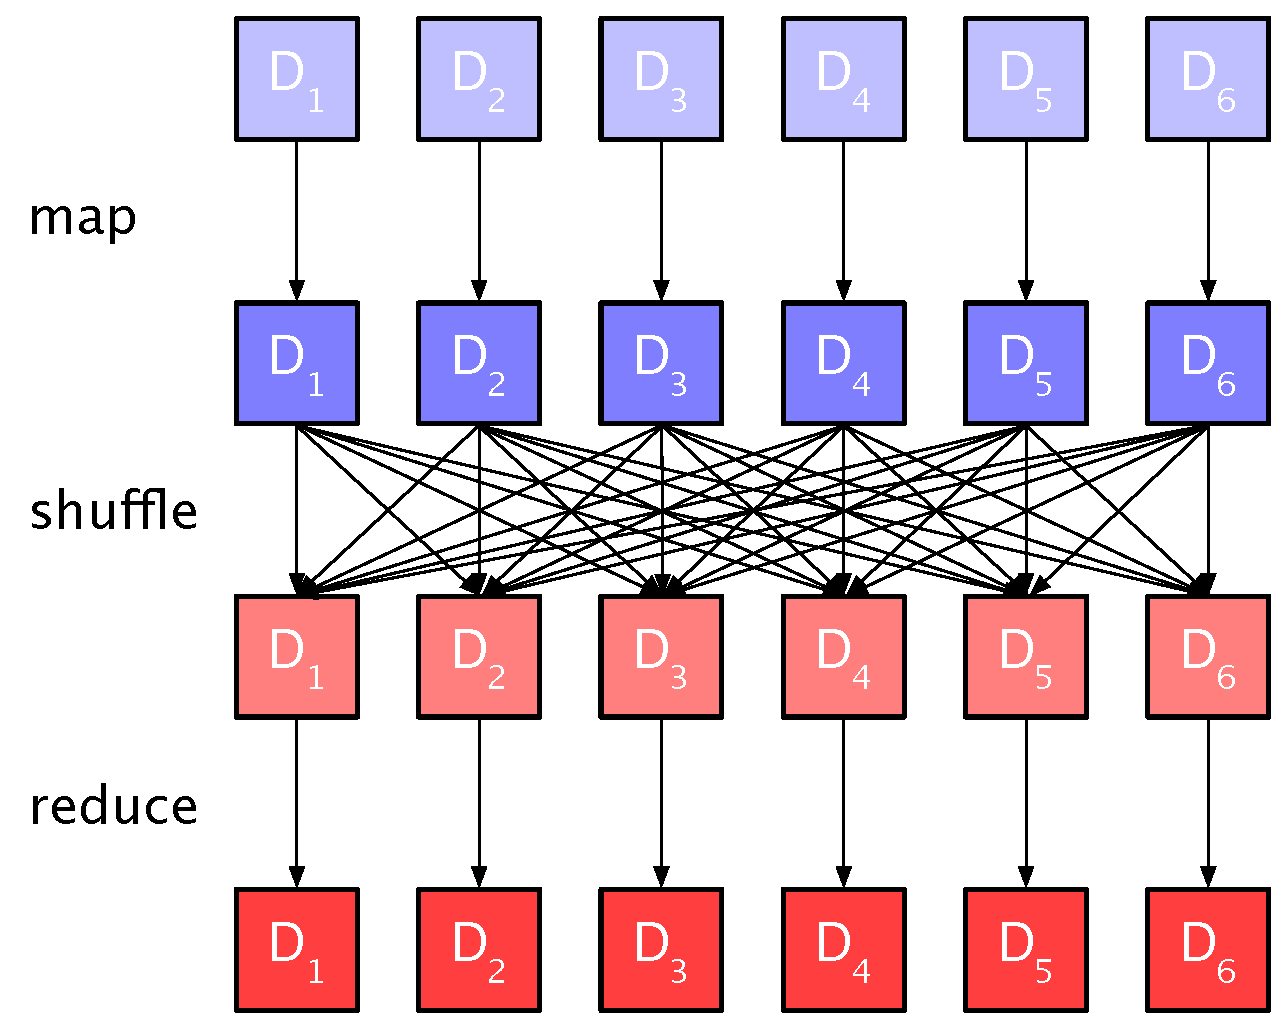
\includegraphics[width=.8\linewidth]{figures/mrmodel}
  \caption{MapReduce}
  \label{fig:mrmodel}
\end{figure}
\subsubsection{MapReduce}
MapReduce~\cite{mapreduce} computes data in map and reduce operations.
In map, a user-defined function on each data record is executed independently.
After map, results are shuffled and redistributed into different partitions
for reduce. In reduce, it read output from previous map and executes
aggregations for specific subsets of data. MapReduce is a functional
computation model, so no states are stored across computations.
Therefore, states of data are stored in data so all states
in previous computations are necessary
for computations in next one. \fig{mrmodel} shows the idea of MapReduce.

\begin{figure}[tbh]
  \center
  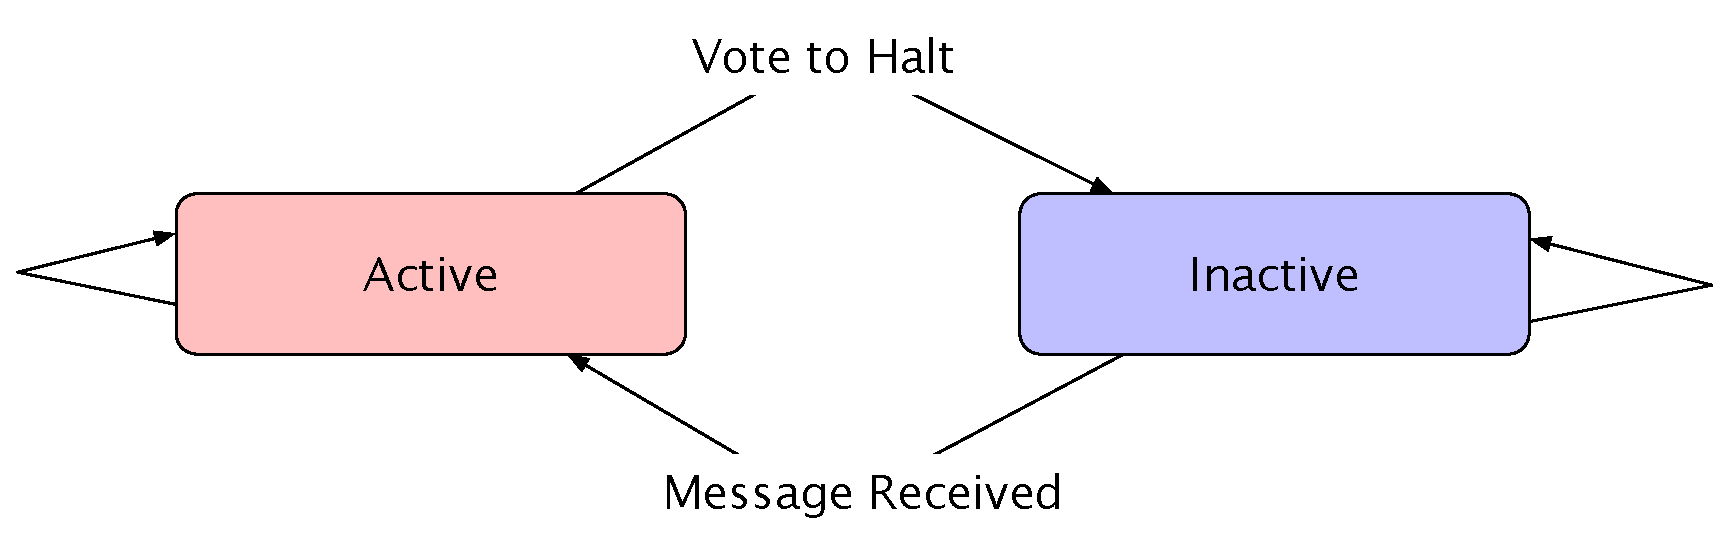
\includegraphics[width=.8\linewidth]{figures/state}
  \caption{The State Machine for Vertices.}
  \label{fig:state}
\end{figure}

\subsubsection{Bulk Synchronous Parallel Model}
The BSP model assumes that computation is done on multiple steps. A bulk contains
some subset of data, and a computation is done on these subset of data. After
computations, the output is used for synchronization.

For graph computing, Pregel makes the BSP model more specific.
Each vertex has two states: active and inactive, and computation
will only be conducted on active vertices. \fig{state} shows the
state machine of a vertex. Computations are done on multiple
supersteps. In the first superstep, all vertices is active and they
will vote to halt and convert to inactive. A vertex will be activate
when a message for the vertex is received.

\begin{figure}
  \center
  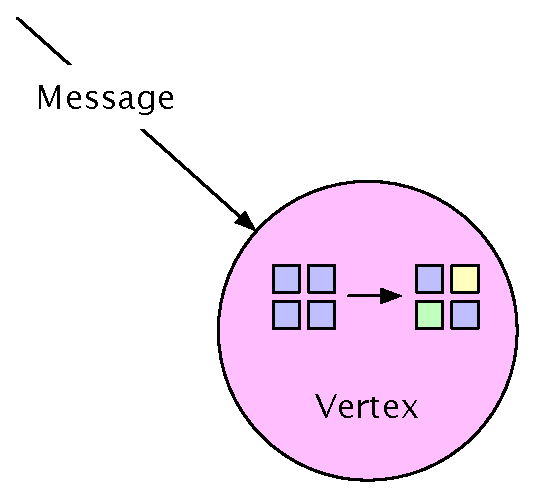
\includegraphics[width=.25\textwidth]{figures/bsp}
  \caption{Bulk Synchronous Parallel (BSP) Model.}
  \label{fig:bsp}
\end{figure}

In each superstep, a vertex get all messages sent to it and computes
result according to the current state of the vertex and sends messages
to its neighbors. \fig{bsp} shows the workflow of BSP.

A Combiner and Aggregator are used for transferring data for message
passing. The Combiner can combines states in each partitions to reduce
network traffics. For example, both vertex $b$ and $c$ send a same
message to vertex $a$, then this message can be combined into one.
On the other hand, Aggregator is used for aggregating output from multiple
vertex and even multiple iterations.

\begin{figure}[tbh]
  \center
  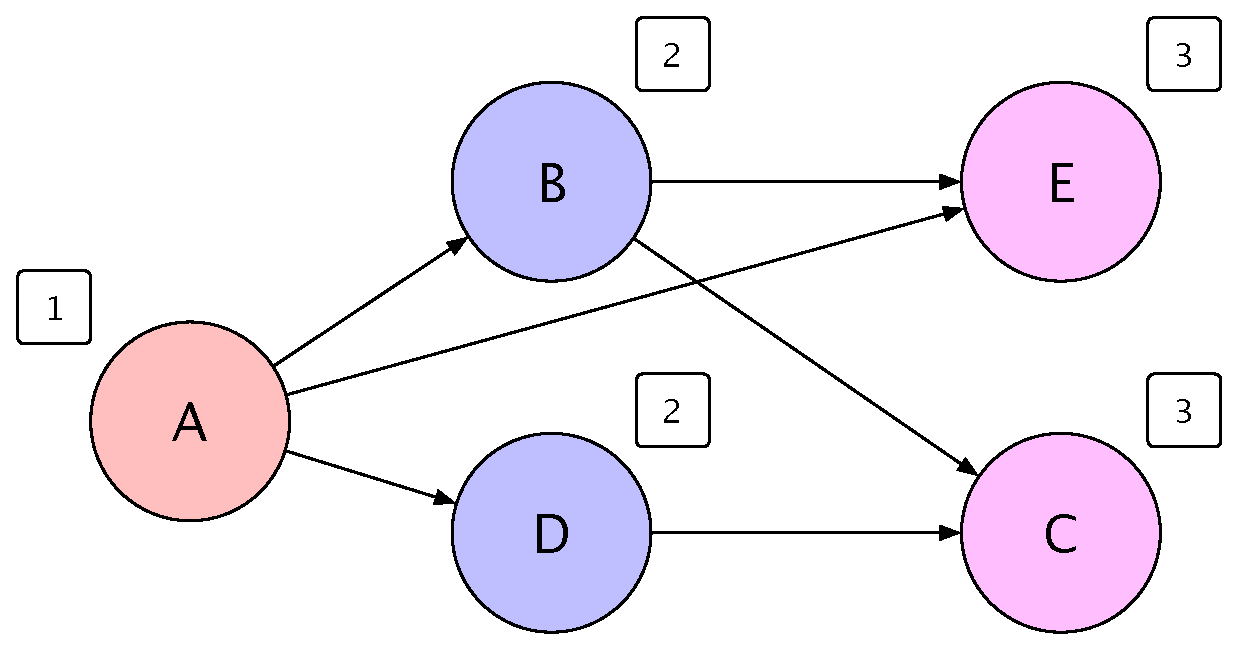
\includegraphics[width=.8\linewidth]{figures/gas}
  \caption{Gather, Apply and Scatter (GAS) model.}
  \label{fig:gas}
\end{figure}

\subsubsection{Gather, Apply and Scatter (GAS) model}
Gather, apply and scatter model (GAS) is more restricted than the BSP model.
Compared with BSP, a vertex in GAS can only interact with neighboring
vertices.

In \textbf{gather} phase, a vertex gathers information from all adjacent vertices, and
set a aggregate function for all the gathered information. Then, it \textbf{apply}
the function and updates values of vertices and edges. At last, in \textbf{scatter},
it can activate it neighboring vertices with information.

Compared with BSP model, a node in GAS only interact with neighboring
vertices. Although it hurts expresses of computations, it also
enable multiple optimization techniques. For example, vertices can
be partitioned and computes in multiple steps (\eg{} using the coring
algorithm). Therefore,
messages passing and computation can be done at the same time, which
greatly improve performance.
Furthermore, a flexible consistency model can be adopted. For example,
a $Vertex Consistency$ only guarantees consistency of read-writes
of vertices. In this cases, races of edges read/writes can happen
and no locking or synchronization are needed, which improve performance.

% Also for GraphLab -> asynchronous execution -> scheduling
% show the graph for consistency and the graph for

\begin{figure}
  \center
  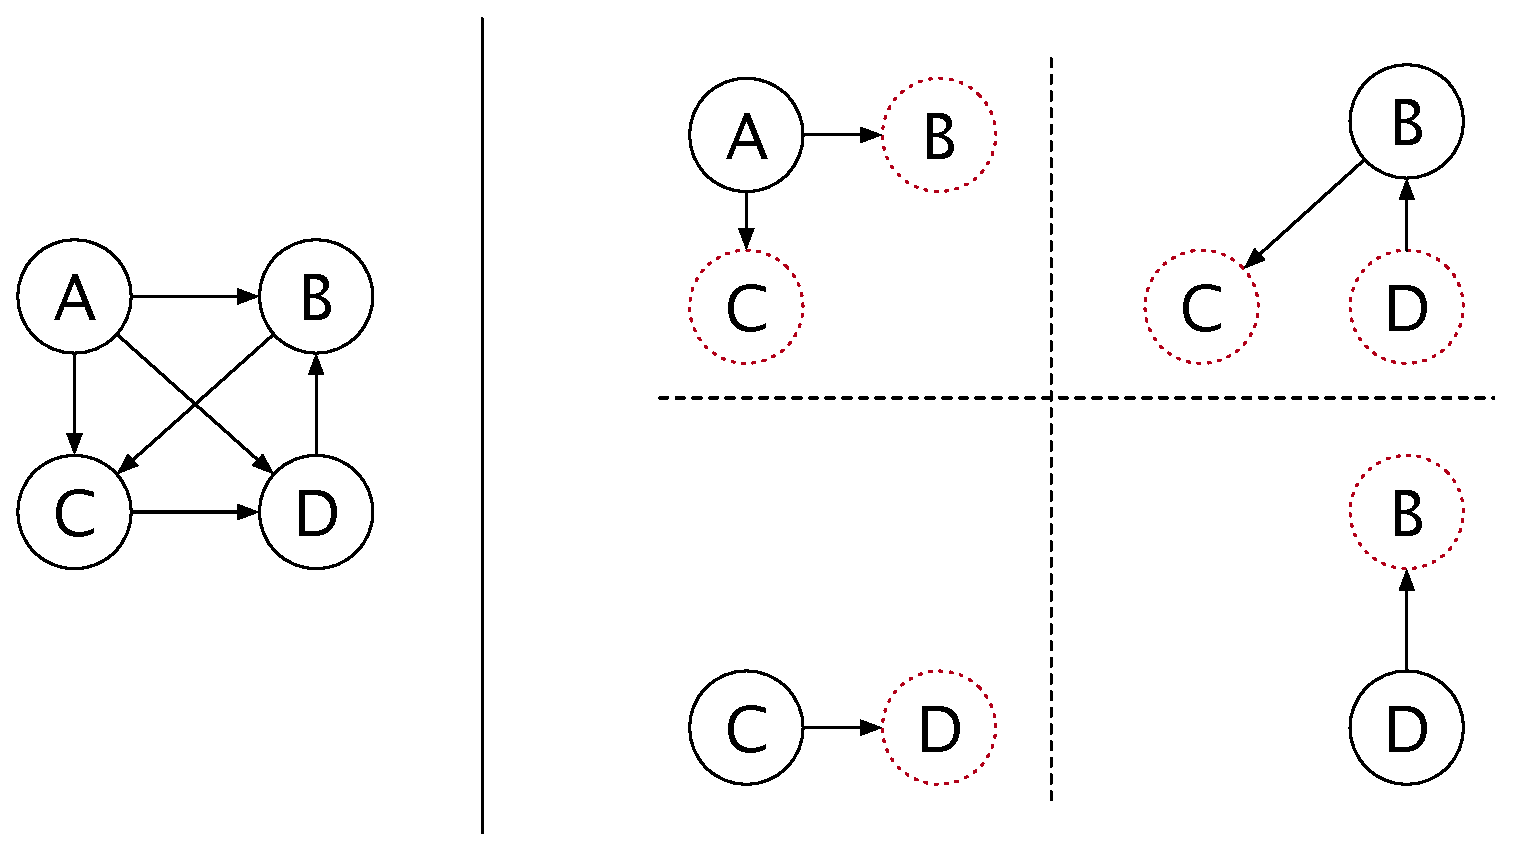
\includegraphics[width=.8\linewidth]{figures/edgecut}
  \caption{Edge Cut approach.}
  \label{fig:edgecut}
\end{figure}

\begin{figure}
  \center
  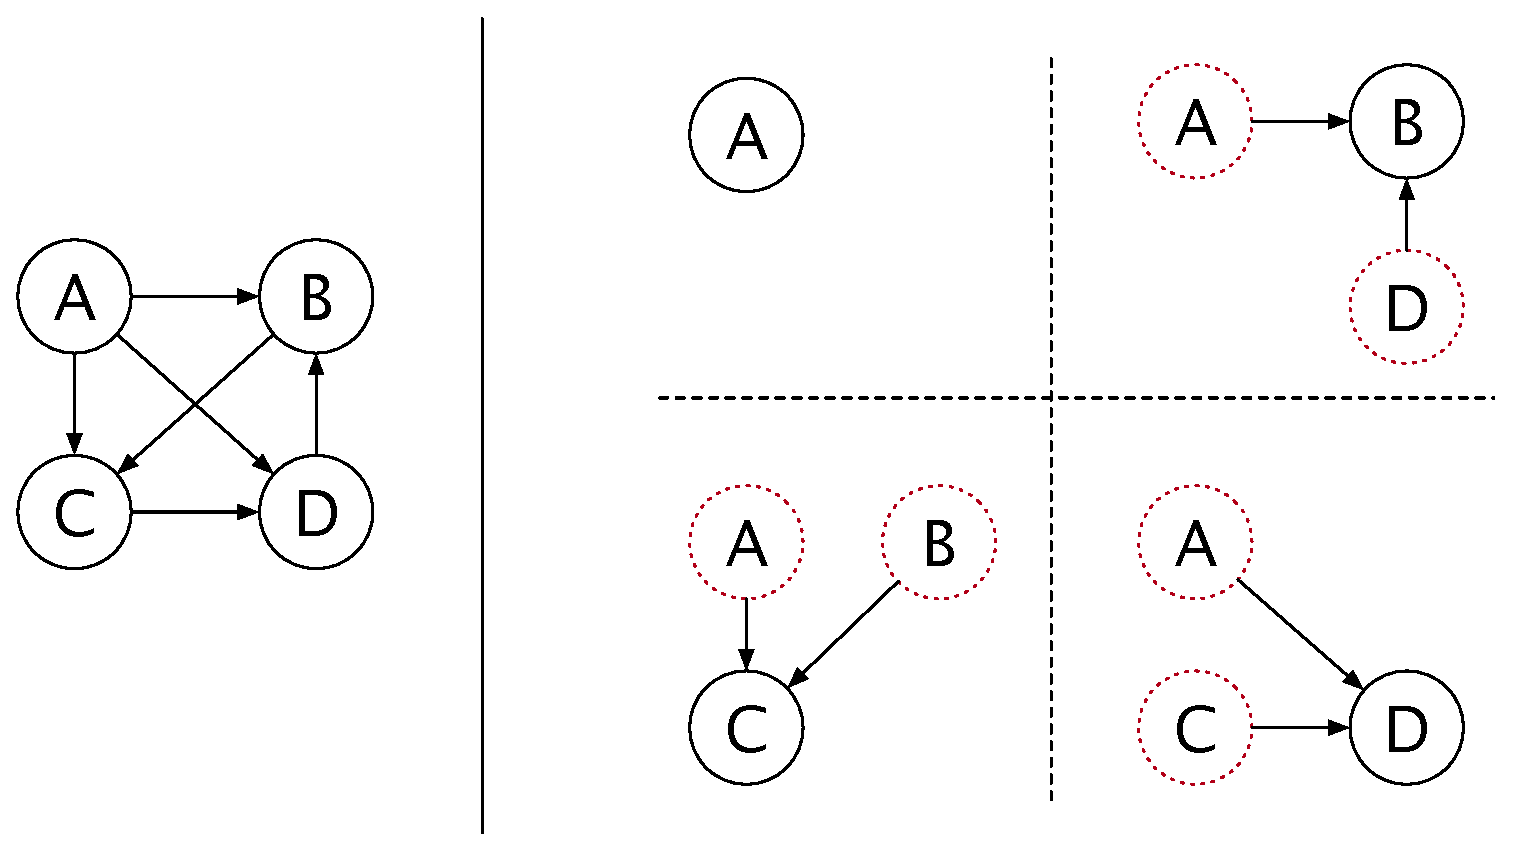
\includegraphics[width=.8\linewidth]{figures/vertexcut}
  \caption{Vertex Cut approach.}
  \label{fig:vertexcut}
\end{figure}

\begin{figure}
  \center
  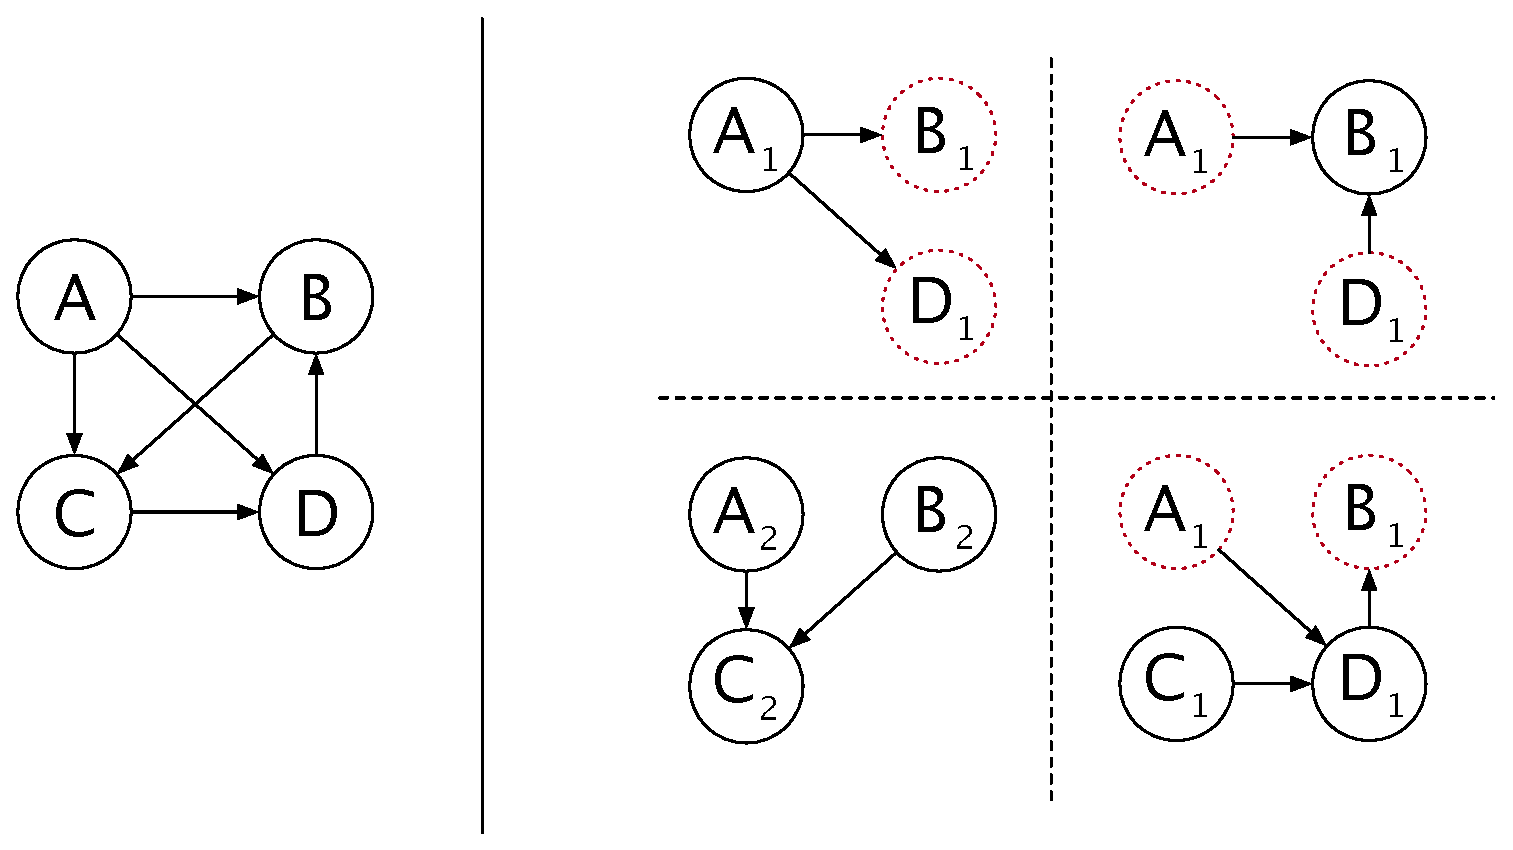
\includegraphics[width=.8\linewidth]{figures/3dcut}
  \caption{3D Cut approach.}
  \label{fig:3dcut}
\end{figure}

\subsection{Partition Scheme}
The way to partition the graph $G$ can greatly affect performance.
The simplest way to partition data is by its vertex id or edge id.
However, this approach incurs too much network traffic. Therefore,
multiple partition schemes have been proposed including \textbf{Vertex Cut},
\textbf{Edge Cut} and \textbf{3D Cut}.
This algorithm is enough for randomly generated
graphs, but for real-world graphs that follow the
power law, a 1D partitioner usually leads to considerable
skewness.\\
\textbf{Vertex Cut} Vertex cut partition vertices into multiple
random partitions. \fig{vertexcut} shows the idea of Vertex Cut. \\
\textbf{Edge Cut} As the Vertex Cut is not suitable for real-life
graph which follows power law, some work~\cite{xstream} propose to partition
data based on edges. In Edge Cut, edges are put into multiple
partitions equally, synchronization of vertices in different nodes
incurs network communications. \fig{edgecut} shows the idea of
Edge Cut. \\
\textbf{3D Cut}
For more, PowerLyra~\cite{powerlyra} use a heristic to combine them.
Cube proposes a new 3D partition of graph, which consider dimensions of data.
Cube~\cite{cube:osdi16} considers the hidden dimensions of vertex partition.
For Machine Learning and Data Mining (MLDM) algorithms, values of vertex
may be linked to values of different vertices. Therefore, different value of a vertex
can be partitioned into different nodes for improved computations. \fig{3dcut}
shows the idea of 3D Cut. \\
\textbf{Dynamic Repartitioning}
Different processes may has imbalance workload, this can hurt performance
as some processes are waiting for result from others. A Dynamic Repartitioning
move data from one node to another so that workload is balanced across
nodes. However, this technique can incur extra network traffics. Moreover,
performance of this technique is not stable, as workload of nodes in next
iterations may change, causing imbalance workloads.\\
\textbf{Mirroring}
To reduce network traffic, Mirroring creates mirroring vertices (or edges)
for a cut edge. Therefore, access of neighboring vertices does not
incur synchronous network messages.
% TODO we need a comparison for different frameworks job stealling and scheduling

% scheduling or concurrency control
